\pdfminorversion=4
\documentclass[aspectratio=169]{beamer}

\mode<presentation>
{
  \usetheme{default}
  \usecolortheme{default}
  \usefonttheme{default}
  \setbeamertemplate{navigation symbols}{}
  \setbeamertemplate{caption}[numbered]
  \setbeamertemplate{footline}[frame number]  % or "page number"
  \setbeamercolor{frametitle}{fg=white}
  \setbeamercolor{footline}{fg=black}
} 

\usepackage[english]{babel}
\usepackage{inputenc}
\usepackage{tikz}
\usepackage{courier}
\usepackage{array}
\usepackage{bold-extra}
\usepackage{minted}
\usepackage[thicklines]{cancel}
\usepackage{fancyvrb}

\xdefinecolor{dianablue}{rgb}{0.18,0.24,0.31}
\xdefinecolor{darkblue}{rgb}{0.1,0.1,0.7}
\xdefinecolor{darkgreen}{rgb}{0,0.5,0}
\xdefinecolor{darkgrey}{rgb}{0.35,0.35,0.35}
\xdefinecolor{darkorange}{rgb}{0.8,0.5,0}
\xdefinecolor{darkred}{rgb}{0.7,0,0}
\definecolor{darkgreen}{rgb}{0,0.6,0}
\definecolor{mauve}{rgb}{0.58,0,0.82}

\title[2024-10-23-chep2024-gil-free-uproot]{GIL-free scaling of Uproot in Python 3.13}
\author{Jim Pivarski}
\institute{Princeton University -- IRIS-HEP}
\date{October 23, 2024}

\usetikzlibrary{shapes.callouts}

\begin{document}

\logo{\pgfputat{\pgfxy(0.11, 7.4)}{\pgfbox[right,base]{\tikz{\filldraw[fill=dianablue, draw=none] (0 cm, 0 cm) rectangle (50 cm, 1 cm);}\mbox{\hspace{-8 cm}\includegraphics[height=1 cm]{princeton-logo-long.png}\hspace{0.1 cm}\raisebox{0.1 cm}{\includegraphics[height=0.8 cm]{iris-hep-logo-long.png}}\hspace{0.1 cm}}}}}

\begin{frame}
  \titlepage
\end{frame}

\logo{\pgfputat{\pgfxy(0.11, 7.4)}{\pgfbox[right,base]{\tikz{\filldraw[fill=dianablue, draw=none] (0 cm, 0 cm) rectangle (50 cm, 1 cm);}\mbox{\hspace{-8 cm}\includegraphics[height=1 cm]{princeton-logo.png}\hspace{0.1 cm}\raisebox{0.1 cm}{\includegraphics[height=0.8 cm]{iris-hep-logo.png}}\hspace{0.1 cm}}}}}

% Uncomment these lines for an automatically generated outline.
%\begin{frame}{Outline}
%  \tableofcontents
%\end{frame}

% START START START START START START START START START START START START START

\begin{frame}[fragile]{What is Python's Global Interpreter Lock (GIL)?}
\Large
\vspace{1 cm}
\begin{onlyenv}<1>
\begin{center}
\includegraphics[height=5 cm]{img/python-gil-meme-1.jpg}
\end{center}
\end{onlyenv}\begin{onlyenv}<2>
\begin{center}
\includegraphics[height=5 cm]{img/python-gil-meme-2.jpg}
\end{center}
\end{onlyenv}\begin{onlyenv}<3>
\begin{center}
\includegraphics[height=5 cm]{img/python-gil-meme-3.png}
\end{center}
\end{onlyenv}\begin{onlyenv}<4>
\begin{minted}{c}
pthread_mutex_lock(&global_interpreter_lock);

PyEval(python_bytecode_instruction);

pthread_mutex_unlock(&global_interpreter_lock);
\end{minted}
\end{onlyenv}\begin{onlyenv}<5>
\includegraphics[width=\linewidth]{img/new_gil.png}

\normalsize
\textcolor{blue}{\url{https://github.com/zpoint/CPython-Internals/blob/master/Interpreter/gil/gil.md}}
\end{onlyenv}
\end{frame}

\begin{frame}{\mbox{ }}
\Large
\vspace{0.5 cm}
\begin{center}
Python 3.13.0 was released 16 days ago.

\vspace{1 cm}
\uncover<2>{It includes two new features for avoiding the GIL.}
\end{center}
\end{frame}

\begin{frame}{Method \#1: subinterpreters}
\large
\vspace{0.5 cm}
\begin{columns}
\column{1.1\linewidth}
\includegraphics[width=\linewidth]{img/thread-interpreter-process.pdf}
\end{columns}

\vspace{0.5 cm}
\uncover<2>{Pre-3.13 trade-off: shared memory + GIL in multithreading or shared-nothing + true parallel-processing in multiprocessing. Now we have an in-between option.}
\end{frame}

\begin{frame}[fragile]{Method \#1: subinterpreters}
\vspace{0.35 cm}
\scriptsize
\begin{minted}{python}
from test.support import interpreters
from test.support.interpreters import queues

def in_subinterp():
    # Need to re-import; this is in its own little world...
    from test.support.interpreters import queues

    in_queue = Queue(in_id)      # in_id comes from global scope
    out_queue = Queue(out_id)    # out_id comes from global scope

    x = queue.get()
    out_queue.put(x + number)    # number comes from global scope

in_queue = queues.create()
out_queue = queues.create()

subinterp = interpreters.create()
subinterp.prepare_main({"in_id": in_queue.id, "out_id": out_queue.id, "number": 42})
subinterp.call_in_thread(in_subinterp)

in_queue.put(100)
assert out_queue.get() == 142
\end{minted}
\end{frame}

\begin{frame}{Method \#1: subinterpreters}
\Large

\begin{center}
Many modules, like NumPy, can't be used in a subinterpreter yet!
\end{center}
\end{frame}

\begin{frame}[fragile]{Method \#2: free-threading}
\vspace{1 cm}
\large

\begin{minted}{bash}
cd Python-3.13.0/
./configure --disable-gil
make
make install
\end{minted}

\vspace{1 cm}
\uncover<2>{Free-threaded Python is a separate ABI, ``{\tt cp313t}'', rather than ``{\tt cp313}''.}

\vspace{0.25 cm}
\uncover<2->{They have to explicitly opt-in to it.}
\end{frame}

\begin{frame}{Free-threaded Python has been discussed for a long time}
\vspace{0.5 cm}
\begin{columns}
\column{1.1\linewidth}
\includegraphics[width=\linewidth]{img/googletrends-gil-timeline.pdf}
\end{columns}

\vspace{0.5 cm}
\uncover<2->{Five forked Pythons, in 2000, 2008, 2013, 2017, 2021, experimentally disabled the GIL.}

\vspace{0.25 cm}
\uncover<3->{Until recently, they all made single (and sometimes multi) threaded performance worse.}
\end{frame}

\begin{frame}{Scaling of pure Python computations}
\vspace{0.5 cm}
\only<1>{\includegraphics[width=0.8\linewidth]{img/scaling-of-compute-basic.pdf}}\only<2>{\includegraphics[width=0.8\linewidth]{img/scaling-of-compute-circle.pdf}}\only<3>{\includegraphics[width=0.8\linewidth]{img/scaling-of-compute-extra.pdf}}
\end{frame}

\begin{frame}{CPU versus time in pure Python computations}
\vspace{0.25 cm}
\begin{center}
\begin{onlyenv}<1>
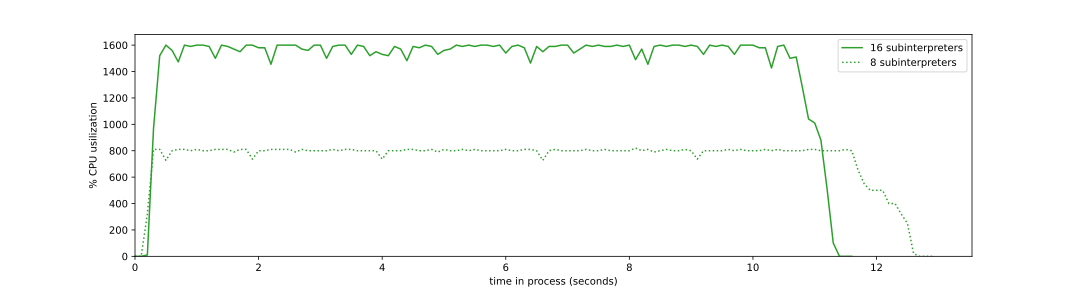
\includegraphics[width=0.93\linewidth]{img/cpu-of-compute-subinterpreters.pdf}

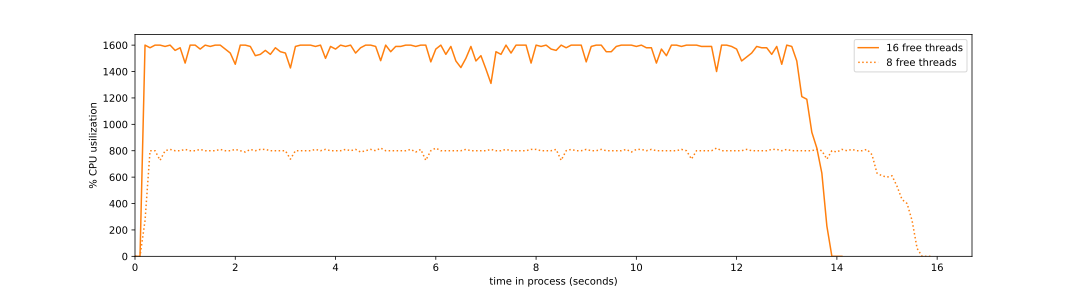
\includegraphics[width=0.93\linewidth]{img/cpu-of-compute-free-threads.pdf}
\end{onlyenv}\begin{onlyenv}<2>
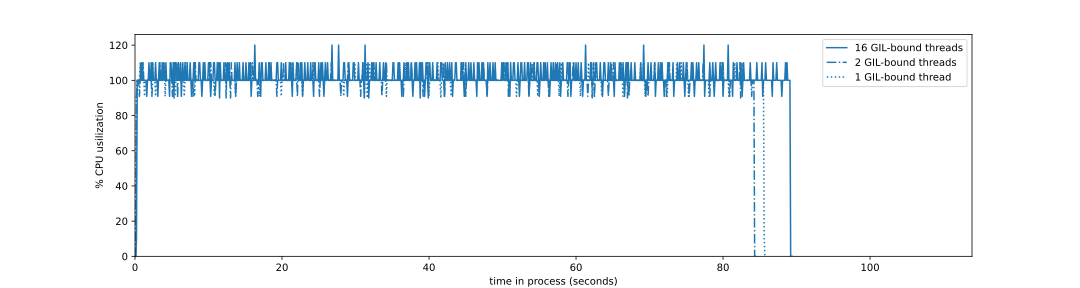
\includegraphics[width=0.93\linewidth]{img/cpu-of-compute-gil-threads.pdf}
\end{onlyenv}
\end{center}
\end{frame}

\begin{frame}{Scaling of pure Python computations (big)}
\vspace{0.5 cm}
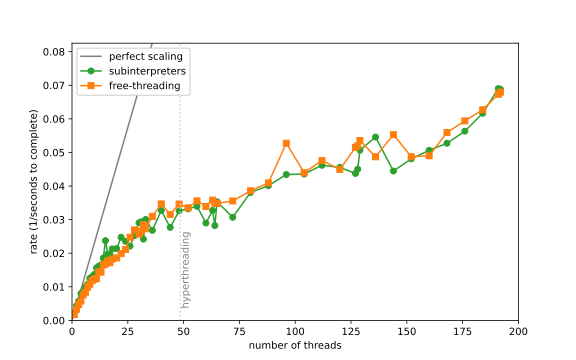
\includegraphics[width=0.8\linewidth]{img/scaling-of-compute-big.pdf}
\end{frame}

\begin{frame}{CPU versus time in pure Python computations (big)}
\vspace{0.25 cm}
\begin{center}
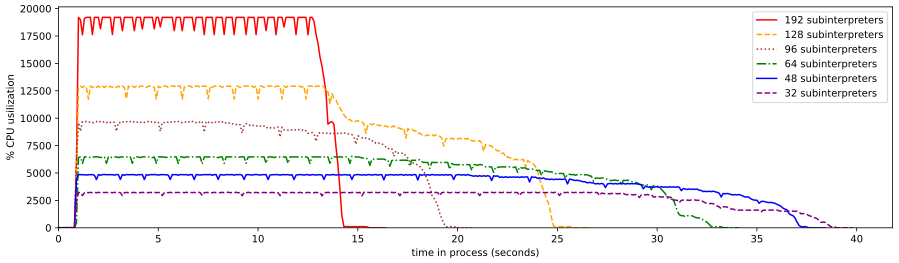
\includegraphics[width=0.93\linewidth]{img/cpu-of-compute-subinterpreters-big.pdf}

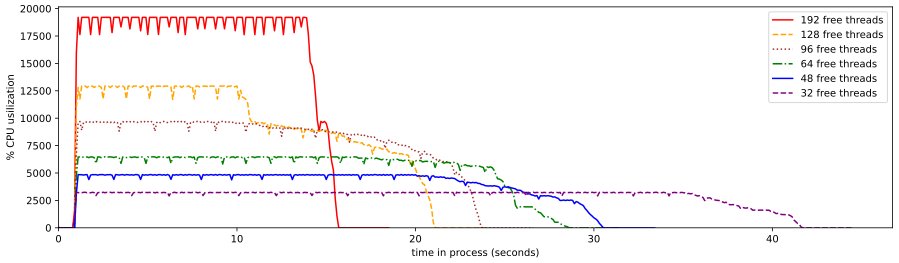
\includegraphics[width=0.93\linewidth]{img/cpu-of-compute-free-threads-big.pdf}
\end{center}
\end{frame}

\begin{frame}{Parallelizing Uproot ``externally''}
\vspace{0.5 cm}
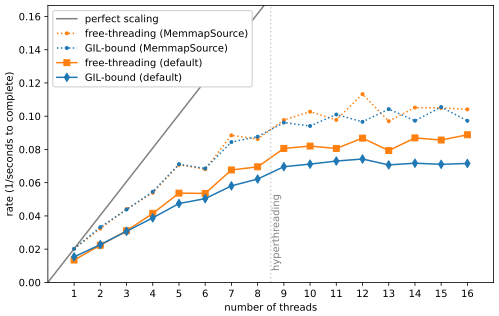
\includegraphics[width=0.8\linewidth]{img/scaling-of-uproot-external.pdf}
\end{frame}

\begin{frame}{Parallelizing Uproot ``internally''}
\vspace{0.5 cm}
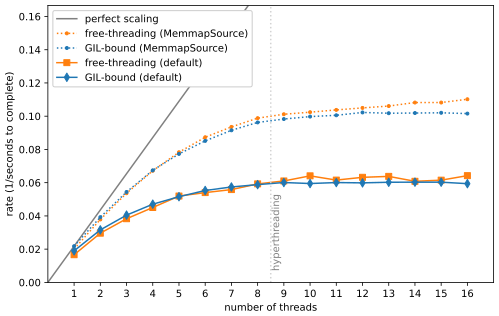
\includegraphics[width=0.8\linewidth]{img/scaling-of-uproot-internal.pdf}
\end{frame}

\begin{frame}{CPU versus time for Uproot (``internal'')}
\vspace{0.25 cm}
\begin{center}
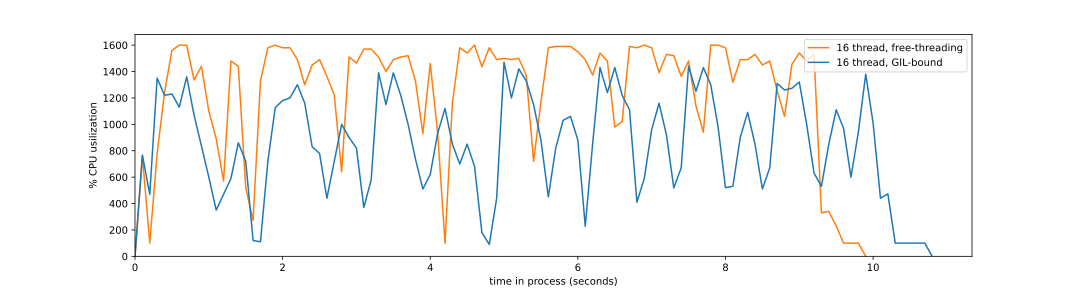
\includegraphics[width=0.93\linewidth]{img/cpu-of-uproot-internal-16.pdf}
\end{center}
\end{frame}

\begin{frame}{Big parallelization of Uproot (``internal'')}
\vspace{0.5 cm}
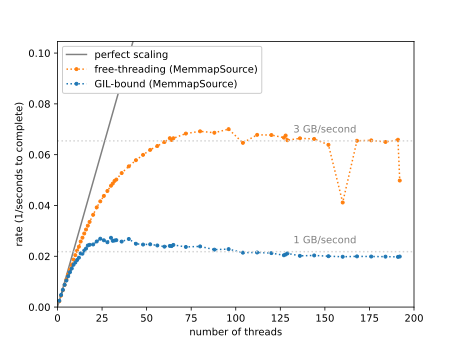
\includegraphics[width=0.8\linewidth]{img/scaling-of-uproot-internal-big.pdf}
\end{frame}

\begin{frame}{CPU versus time for Uproot (``internal'')}
\vspace{0.25 cm}
\begin{center}
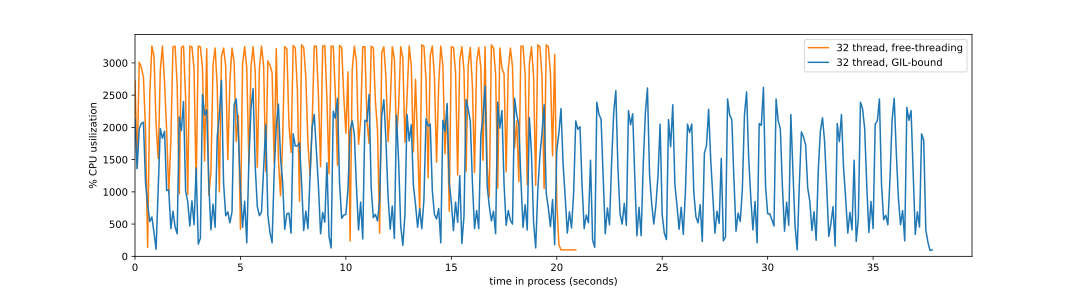
\includegraphics[width=0.93\linewidth]{img/cpu-of-uproot-internal-big-32.pdf}

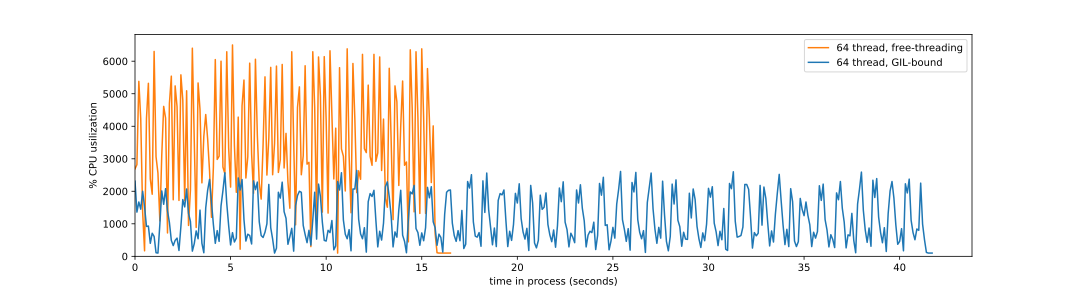
\includegraphics[width=0.93\linewidth]{img/cpu-of-uproot-internal-big-64.pdf}
\end{center}
\end{frame}



\end{document}
